\documentclass{article}

\usepackage[utf8]{inputenc}
\usepackage[T1]{fontenc}
\usepackage[english]{babel}
\usepackage{amsmath}
\usepackage{amssymb}
\usepackage{lmodern}
\usepackage{todonotes}
\usepackage{fullpage}
\usepackage{fancyhdr}
\usepackage[Glenn]{fncychap}
\usepackage{theorem}
\usepackage{hyperref}
\usepackage{tikz}
\usepackage{float}

\usepackage{appendix}

%%%%%%%%%%%%INCLUDE R CODE
\usepackage{listings}
\lstset{
	language=R,
	basicstyle=\scriptsize\ttfamily,
	commentstyle=\ttfamily\color{blue},
	numbers=left,
	numberstyle=\ttfamily\color{gray}\footnotesize,
	stepnumber=1,
	numbersep=5pt,
	backgroundcolor=\color{white},
	showspaces=false,
	showstringspaces=false,
	showtabs=false,
	frame=single,
	tabsize=2,
	captionpos=b,
	breaklines=true,
	breakatwhitespace=false,
	title=\lstname,
	escapeinside={},
	keywordstyle={},
	morekeywords={}
}
%%%%%%%%%%%%
%\hypersetup{backref, pdfpagemode=FullScreen, colorlinks=true, linkcolor={blue}}
%\usepackage[]{color}
\setlength{\headheight}{15.5pt}
\title{Project in Applied Econometrics\\ Report}
\author{Lucas Javaudin, Robin Le Huérou-Kérisel, Rémi Moreau}
\date{March 2018}

\begin{document}
\maketitle

%notes:
%art et essai: impact sur la taille du réseau ou sur la précision du prix (plus de social learning?)
%ne pas inclure moyenne spectateurs dans la reg
%
%Quelques éléments à inclure dans le rapport:
%-présentation du modèle (<5 pages, il faut vulgariser le modèle pour que quelqu'un qui ne connait pas le modèle puisse le comprendre --déjà fait en partie dans le mid-term report)
%-présentation des jeux de données
%-expliquer des parties intéressantes du code
%-graphiques intéressants (?)
%-prendre exemple sur l'article de Moretti
%-critiques intéressantes (les variables utilisées par Moretti -- explications parfois douteuses ou manquant de justifications scientifiques)
%
%
%-mettre en parrallèle les régressions et les résultats
%-donner les résultats intéressants
%-test de student pour la convexité et concavité
%
%
%Pour Robin:
%sec1: comment trouve-t-on les surprises
%sec2: surprises and sale dynamics
%sec3: precision of the prior
\begin{abstract}
	This project aims at reproducing a paper by Moretti (2011) on social learning effects in movie sales with R. We then confront his theory and predictions with French data. We find evidence of social learning in French movie sales but our results are less robust than the results of Moretti.
\end{abstract}
\tableofcontents
\pagebreak
\section{Intuitions and Detailed Presentation of the Model}

\subsection{Some intuitions}

\subsection{Presentation of the model}




Moretti develops a model that defines social learning as the effect of one consumer's opinion on a given good's consumption, on her acquaitancies's willingness to consume.\\
Applied to cinema, his idea is that comsumers go and see a certain film if they get a sufficient expected utiliy to compensate the cost of viewing.\\
\subsection{Utility Estimation Before A Movie Is Released}	
\subsubsection{Actual Utility}
The utility provided by a given film (called "quality") is estimated by the consumers before the movie is being launched. They use the the objective elements about the film, available to them all, to get a \textit{prior}. Consumers also get a personal \textit{signal} that indicates how much they are attracted by the film's concept.\\
\\
Expected utility is the weighted average of the prior and the signal. Progressively, the acquaintancies' opinion on the film is also included in this weighted average. \\
\\
An individual i gets a utility $U_{i,j}$ watching the film j with\\
\begin{equation} \label{eq:1}
	U_{i,j}=\alpha_{j}^{*}+v_{i j},
\end{equation}
where $\alpha_{j}^{*}$ is the quality of the movie for the average individual and $v_{i j}\sim \mathcal{N}(0,\frac{1}{d})$ represents how much individual i's appeal for movie j differs from the the average individual's taste for this movie (that is the reason why the variable $v_{i j}$ is zero-mean).\\
\\
It is worth noticing that $v_{i j}$'s variance is independant of both i and j: the distribution of the tastes aroung the mean is supposed to be constant (in absolute value) no matter the film.\\
\\
These two parameters are supposed to be unobserved. This is consistent for $\alpha_{j}^{*}$ as an individual may find it hard to estimate precisely the advice of the \textit{average consumer}: she does not observe all advices, thus cannot precisely determine the mean of all the tastes. So $\alpha_{j}^{*}$ can be considered as a random variable; to make the model rather simple, this variable is supposed to be normal, i.e. totally characterized by its mean and variance.\\
\\
This variable's mean (referred to precedently as the prior) can be estimated from all the observable features of the film (such as the director, the budget, the casting...), that are aggregated into the variable $X_{j}$. Thus, $\mathbb{E}(\alpha_{j}^{*})=X_{j}'\beta$, like in a simple linear model. This expression embodies one of Moretti's key ideas in his paper, that a film's quality is the only determiner of the utility if we omit interpersonal differences in tastes.\\
$\alpha_{j}^{*}$'s variance does not depend on the individual doing the estimation (all individual are supposed to have the same information about the film and to analyse it the same way). Nevertheless, it depends on the movie. Sequels and films shot by famous directors are characterised by a much lower variance since the precedent movies'outcome (success or failure) could be observed.\\
Thus: $\alpha_{j}^{*}\sim \mathcal{N}(X_{j}'\beta,\frac{1}{m_{j}})$\\
	
\subsubsection{Signal: Noisy Utility}
Moretti suposes that consumers don't measure $u_{i,j}$ but recieves instead a noisy signal
\begin{equation*}
	s_{i j}=U_{i j}+\epsilon_{i j}, \;\epsilon_{i j}\sim \mathcal{N}(0,\frac{1}{k_{j}}).
\end{equation*}
Introducing an unbiased signal allows that the averages of s and U are the same for a certain movie j, which is a basic requirement in a social learning model (aggregated signal gives an unbiased estimator). Additionnaly, for a set of movies that give the same utility to a given consumer and that have the same variance for $\epsilon_{i j}$, the consumer makes on average correct predictions of her utility starting from the signal she gets. \\
$\epsilon_{i j}$ and $v_{i j}$ are also supposed independant of each other and of $\alpha_{j}^{*}$; the idea is that the objective quality of the film, the subjective appeal for it and the error in measuring these values aren't correlated, since they are of different nature.\\
It is worth noticing, in that sense, that the three variables introduced above are all considered as random, but in different senses. For  $\alpha_{j}^{*}$ it can be interpreted as a lack of sufficient information to estimate $\beta$ correctly. For $v_{i j}$ the probability distribution allows to consider a set of different individuals with different tastes. $\epsilon_{i j}$ is rather an error of interpretation (or, more mathematically, of measurement) during the determining of $U_{i j}$\\\\
Additionaly we suppose that $X_{j}$, $\beta$, $m_{j}$, $k_{j}$ and d are well-known by all the consumers.
\\
\subsubsection{Expected Utiliy}
As said above, the exprected utiliy in the first week (i.e. before the film is being released) is estimated by the weighted average of the prior and the signal, namely:
\begin{center}
	$\mathbb{E}_1[U_{i j}|X_{j}'\beta, s_{i j}]=\omega_{j} X_{j}'\beta+(1-\omega_{j})s_{i j}$.
\end{center}
The idea is to use to different estimators of $U_{i j}$: its estimated average value (which is certain) and its value with some zero-mean noise (which cumulates several uncertainties).\\
The expression of the variance has to put more weight on the most precise term between the two estimators of $U_{i j}$; we want to know whether it is better \\
- to omit widely the personal part $v_{i j}$ (of variance $\frac{1}{d})$) and the error in estimating the average value $\alpha_{j}^{*}$ (of variance $\frac{1}{m_{j}})$), i.e. to put more weight on $X_{j}'\beta$,\\
- or to cope with noise $\epsilon_{i j}$ (of variance $\frac{1}{k_{j}}$), i.e. to put more weight on $s_{i j}$.\\
\\
Like in the WLS approach, we minimize the exprected value of the square difference between the right-hand side above, and the sought term $U_{i j}$, choosing the optimal $\omega_{j}$, i.e. :
\begin{center}
	$\min_{\omega_{j}} \mathbb{E}((\omega_{j} X_{j}'\beta+(1-\omega_{j})s_{i j}-U_{i j})^{2})=\min_{\omega_{j}} \mathbb{E}((-\omega_{j} (\alpha_{j}^{*}-X_{j}'\beta+v_{i j})+(1-\omega_{j})\epsilon_{i j})^{2})$.
\end{center}
The solution is, according to Appendix 1:
\begin{center}
	$\omega_{j}(\frac{1}{h_{j}}+\frac{1}{k_{j}})=\frac{1}{k_{j}}$
	$\omega_j=\frac{h_{j}}{h_{j}+k_{j}}$.
\end{center}
with $h_{j}=\dfrac{1}{\frac{1}{d}+\frac{1}{m_{j}}}=\frac{d m_{j}}{d+m_{j}}$ ($h_{j}=Var(U_{i j})$ too)
Thus:
\begin{equation}
\mathbb{E}_1[U_{i j}|X_{j}'\beta, s_{i j}]=\omega_{j} X_{j}'\beta+(1-\omega_{j})s_{i j}, \omega_j=\frac{h_{j}}{h_{j}+k_{j}}, h_{j}=\frac{d m_{j}}{d+m_{j}}
\end{equation}
\\
\subsubsection{Cost Of Watching}
In the model, a consumer decides to go and watch a film if her utility is higher than her subjective cost of watching in the week considered (parameter t), depending for example on whether she has a lot or a few activities planned during the week: 
\begin{equation}
	\mathbb{E}_1[U_{i j}|X_{j}'\beta, s_{i j}]>q_{i t}
\end{equation}
To model the idea that the cost depends on the individual and on the week, Moretti supposes that $q_{i t}=q+u_{i t}$ with $u_{i j}\sim \mathcal{N}(0,\frac{1}{r})$ with all $u_{i t}$ independant. $u_{i t}$ is zero-mean so the cost of watching has the same average value (between individuals) every week, and the same average for a given individual during a long period of time. As a consequence, the consumers are considered similar; the stuctural difference of timetable between positions and jobs is not taken into account, or it is supposed not to influence the possibility to go to the movies.\\
\\
\subsubsection{Probability Of Watching}
To finish with, let us compute the probability for individual i to go to see movie j in the first week. To do so, we will have to change the viewpoint, from the consumer deciding whether or not to see a movie, to an observer of the market looking at the result of consumer's decision at an aggregate level. The aim is to get a formula that is possible to use. More precisely, all variables with indexes 'i' won't be observable any more, but the average $\alpha_{j}^{*}$ is now obervable (thus precisely determined); this induces a certain form for the result. The sought probability of watching is in this context:
\begin{equation} \label{eq:4}
	P_{1}=\mathbb{P}(\mathbb{E}_1[U_{i j}|X_{j}'\beta, s_{i j}]>q_{i t})=\Phi\left(\frac{(1-\omega_{j})(\alpha_{j}^{*}-X_{j}'\beta)+X_{j}'\beta-q}{\sigma_{j 1}}\right),
\end{equation}
\begin{align*}
	\sigma_{j 1}^{2}=(1-\omega_{j})^{2}\left(\frac{1}{k_{j}}+\frac{1}{d}\right)+\frac{1}{r}
\end{align*}
with $\Phi$ is the cumulative function of a standard normal distribution $\mathcal{N}(0,1)$
Moretti underlines that the term $\alpha_{j}^{*}-X_{j}'\beta$ that appears in the previous equation measures the surprise. It is indeed the difference between\\
- the 'true quality' of the movie $\alpha_{j}^{*}$, in the sense of average utility that consumers get by viewing the film, that only the observer of the market sees, and\\
- $X_{j}'\beta$, the prior of quality, which is the only piece of information movie theatres have and one of the only two consumers have to estimate the quality of the movie. The observer of the market can also see it.\\
\\
The expression 'surprise' is justified by the fact that a positive difference $\alpha_{j}^{*}-X_{j}'\beta$ increases the probability of watching and conversely. The presence of this term is justified by the fact that\\
- movie theatres have less information than consumers\\
- both information consumers recieve are unbiased\\
- consumers are numerous and thus, on average, the utility they expect is close to the true utility (or quality) $\alpha_{j}^{*}$, which is totally determined by the consumer's appeal for the film.\\
\\
With neither social learning, nor decrease in utility for viewing a film again and again, the previous formula for $P_{1}$ remains valid as long as the movie can be watched.\\
	
\subsection{Utility Estimation With Social Learning}	
	
\subsubsection{Signal With Feedback}
Let us add social learning in the model now. In week 2, we consider a consumer i who has $N_{i}$ peers, $n_{i}$ of which see the movie in Week 1. They all give their utiliy $U_{p j }$, $p\in[1,n_{i}]$ as a feedback to i after watching. Consumer i recieves two information in the same time:\\
- the fact that his acquaintancies who saw the film had a sufficiently high expected (ex-ante) utility to do so, i.e.:
\begin{align*}
	\omega_{j} X_{j}'\beta+(1-\omega_{j})s_{p j}>q_{p 1},
\end{align*}
and that the $N_{i}-n_{i}$ other peers did not verify such inequality.\\
- and their ex-post utility itself.\\\\
By maximum likelihood estimation we obtain an estimate $S_{i j 2}$ such that (see Appendix 3):
\begin{equation}
	S_{i j 2}=\frac{1}{n_{i}}\sum_{p=1}^{n_{i}}U_{p j}-\frac{1-\omega_{j}}{d\sigma_{V}}\frac{N_{i}-n_{i}}{n_{i}}\frac{\phi\left(\frac{q-\omega_{j}X'_{j}\beta-(1-\omega_{j})S_{i j 2}}{\sigma_{V}}\right)}{\Phi\left(\frac{q-\omega_{j}X'_{j}\beta-(1-\omega_{j})S_{i j 2}}{\sigma_{V}}\right)}\\
\end{equation}
	
The second part of the expression is negative so that $S_{i j 2}$ is lower than the average of the ex-post utilities consumer i recieves; this is the impact of non-viewers.\\
	
Moretti underlines that the estimator obtained is unbiased and asymptotically normal (this second property comes from the fact that the estimator is a likelihood maximizer): 
\begin{equation}
	S_{i j 2}\sim\mathcal{N}(\alpha_{j}^{*}, \frac{1}{b_{i 2}}) , b_{i 2}=dn_{i}+(N_{i}-n_{i})\frac{\phi(c)}{\Phi(c)}\left(c+\frac{\phi(c)}{\Phi(c)}\right)(\frac{1-\omega_{j}}{\sigma_{V}})^{2}
\end{equation}\\
	
\subsubsection{Expected Utility}
Consumer i will do a weighted average of the three information she has, $X_{j}'\beta, s_{i j}$ and $S_{i j 2}$, just like in the first week:
\begin{equation}
	\mathbb{E}_2[U_{i j}|X_{j}'\beta, s_{i j}, S_{i j 2}]=\frac{h_{j}}{h_{j}+k_{j}+z_{i 2}} X_{j}'\beta+\frac{k_{j}}{h_{j}+k_{j}+z_{i 2}}s_{i j}+\frac{z_{i 2}}{h_{j}+k_{j}+z_{i 2}}S_{i j 2}, 
\end{equation}
\begin{align*}
	h_{j}=\frac{d m_{j}}{d+m_{j}}, z_{i 2}=\frac{b_{i 2}d}{b_{i 2}+d}.
\end{align*}
Likewise, in week $t\geqslant2$, the exprected utility is
\begin{align*}
	\mathbb{E}_t[U_{i j}|X_{j}'\beta, s_{i j}, S_{i j 2}, ..., S_{i j t}]=\frac{h_{j}X_{j}'\beta}{h_{j}+k_{j}+\sum_{s=2}^{t}z_{i s}} +\frac{k_{j}s_{i j}}{h_{j}+k_{j}+\sum_{s=2}^{t}z_{i s}}+\sum_{w=2}^{t}\frac{z_{i w}S_{i j 2}}{h_{j}+k_{j}+\sum_{s=2}^{t}z_{i s}}, 
\end{align*}
\begin{equation}
	\mathbb{E}_t[U_{i j}|X_{j}'\beta, s_{i j}, S_{i j 2}, ..., S_{i j t}]=\omega_{j 1 t}X_{j}'\beta +\omega_{j 2 t}s_{i j}+\sum_{w=2}^{t}\omega_{j 3 w}S_{i j w}, 
\end{equation}
\begin{align*}
	\omega_{j 1 t}=\frac{h_{j}}{h_{j}+k_{j}+\sum_{s=2}^{t}z_{i s}}, 
	\omega_{j 2 t}=\frac{k_{j}}{h_{j}+k_{j}+\sum_{s=2}^{t}z_{i s}}, 
	\omega_{j 3 w}=\frac{z_{i w}}{h_{j}+k_{j}+\sum_{s=2}^{t}z_{i s}},\\
	h_{j}=\frac{d m_{j}}{d+m_{j}}, z_{i t}=\frac{b_{i t}d}{b_{i t}+d}.
\end{align*}
	
This equation shows that a given piece of information has a decreasing importance in the final decision from week to week.\\
	
\subsubsection{Probability of Watching}
Just like before, the probability of watching at week t is (see Appendix 4):
\begin{align*}
	P_{t}&=\mathbb{P}(\mathbb{E}_t[U_{i j}|X_{j}'\beta, s_{i j}, S_{i j 2}, ..., S_{i j t}]>q_{i t})\\
	&=\Phi\left(\frac{(1-\omega_{j 1 t})(\alpha_{j}^{*}-X_{j}'\beta)+X_{j}'\beta-q}{\sigma_{j t}}\right),
\end{equation}
with:
\begin{align*}
	\sigma_{j t}^{2}
	&=(\omega_{j 2 t })^{2}\left(\frac{1}{k_{j}}+\frac{1}{d}\right)+\frac{\sum_{p=2}^{t}z_{i p}}{(h_{j}+k_{j}+\sum_{s=2}^{t}z_{i s})^{2}}+\frac{1}{r}
\end{align*}
	
To analyze this equation we can consider first the case $X_{j}'=\alpha_{j}^{*}$ (no surprise). Then $P_{t}=\Phi\left(\frac{X_{j}'\beta-q}{\sigma_{j t}}\right)$: the higher the difference between the prior and the average cost (average for every week and/or every consumer), the higher the probability for a viewer to watch the film, and thus the higher the attendance to see the movie considered. The probability of viewing is constant equal to one-half when $X_{j}'\beta=q$.\\
To study the evolution over time we can derivate (discretely) $P_{t}$ two times w.r.t t. When $X'\beta=q$, we obtain (in Appendix 5) a consistent model, as announced by Moretti, if some condition is verified by the parameters ($h_{j}<k_{j}$ or $h_{j}<\frac{2k_{j}^{2}}{d}$ is sufficient): if we have a positive surprise, i.e. $\alpha_{j}^{*}>X_{j}'\beta$, the the probability of going to watch the film is increasing from one week to the following, whereas a negative surprise $\alpha_{j}^{*}<X_{j}'\beta$ leads to a decrease in this probability across the weeks. Additionaly, without any surprise, i.e. $\alpha_{j}^{*}=X_{j}'\beta$, the probability of watching in constant over time.\\
Moretti underlines that the second derivative has the opposite sign from the first derivative, meaning that:
\begin{center}
	$\frac{\partial ^{2} P_{t}}{\partial t^{2}}<0$ (concavity) when $\alpha_{j}^{*}>X_{j}'\beta$ and $\frac{\partial ^{2} P_{t}}{\partial t^{2}}>0$ (convexity) when $\alpha_{j}^{*}<X_{j}'\beta$.
\end{center}
The concavity or convexity is the mark of a social learning multiplier: from one week to another, the quality becomes more and more precisely known, additional advice from peers bring marginally less and less information from one week to another.\\
If we relax the hypothesis $X'\beta=q$, the same tendancies are observed but with a threshold. Considering again the sufficient conditions above, when $X'\beta>q$, the prior on quality of the movie exceeds the cost of viewing, so the impact of a negative surprise on the probability of watching the film is lower. This is due to the fact that people, in that case, are to perform a trade-off between a strongly positive prior and a negative surprise. We have a symetric situation when $X'\beta<q$ and people's signal shows a negative surprise.
	
\subsubsection{Ruling Out Nework Externalities}
Moretti wants to show a social learning effect and to rule out a network externality effect. The latter is present when a consumer has a utility that depends only on the number of people who have watched the film (for example, so as to speak with them about the film). The theory he develops models the idea that the evolution in sales is due to the process of estimation of a movie's quality, and not merely on the attendance for a given movie.

\pagebreak
\section{Analysis and Main Results}

%sec1: comment trouve-t-on les surprises
%sec2: surprises and sale dynamics
%sec3: precision of the prior

%Sales of movies with positive surprise and sales of movies with negative surprise should diverge over time. To test this, we need to regress the log of sales on time and the interaction between time and surprise. If the coefficient of the interaction between time and surprise is significantly positive, then the sales of movies with positive surprise decrease slower than the sale of movies with negative surprise. If our results are consistent with those of Moretti, we should find that controlling for advertising, critic reviews and other variables does not affect significantly the results.

% The effect of a surprise should be lower for movies with a more precise prior. To test this, we augment the previous regression equation with the interaction of time and the precision of the prior and the interaction of time, precision of the prior and surprise of the movie (whose coefficient is predicted to be negative). The precision of the prior can be a dummy for sequels (sequels are assumed to have a more precise prior) or can be measured by the variance of the first week surprise for movies of the same genre.

\subsection{Identification of the surprises}

Surprises consist in the residuals of the regression of the log-number of sales in the first week on the log-number of screens available (opened by theaters). This definition of surprises holds because we suppose that theaters are profit-maximizing agents and make use of all the available information to predict the success of a movie. If this definition is correct, we should expect log-number of screens opened by theaters first week to be a good indicator of knowledge available on the movie quality before it is released. In the Table \ref{part2.1_tab1} we reproduce Moretti's regression of \textit{log\_sales\_first\_we} on \textit{log\_screens\_first\_week}. Each column is the result of the regression when we control with some variables (film genre, rating available, cost, distributor, weekday, month, week, year). The fact that adding control variables doesn't change the robustness of the regression proves Moretti's point which is that theaters take into account these factors when deciding their number of available screens. 

\begin{table}[!htbp] \centering 
	\caption{Regression of first-weekend sales on number of screens} 
	\label{part2.1_tab1} 
	\begin{tabular}{@{\extracolsep{5pt}}lccccccc} 
		\\[-1.8ex]\hline 
		\hline \\[-1.8ex] 
		& \multicolumn{7}{c}{\textit{Dependent variable:}} \\ 
		\cline{2-8} 
		\\[-1.8ex] & \multicolumn{7}{c}{log\_sales\_first\_we} \\ 
		\\[-1.8ex] & (1) & (2) & (3) & (4) & (5) & (6) & (7)\\ 
		\hline \\[-1.8ex] 
		log\_screens\_first\_week & 0.893$^{***}$ & 0.896$^{***}$ & 0.883$^{***}$ & 0.871$^{***}$ & 0.803$^{***}$ & 0.806$^{***}$ & 0.813$^{***}$ \\ 
		& (0.004) & (0.005) & (0.005) & (0.005) & (0.006) & (0.006) & (0.006) \\ 
		& & & & & & & \\ 
		\hline \\[-1.8ex] 
		R$^{2}$ & 0.907 & 0.909 & 0.910 & 0.912 & 0.932 & 0.936 & 0.938 \\ 
		Adjusted R$^{2}$ & 0.907 & 0.908 & 0.910 & 0.912 & 0.928 & 0.931 & 0.933 \\ 
		\hline 
		\hline \\[-1.8ex] 
		\textit{Note:}  & \multicolumn{7}{r}{$^{*}$p$<$0.1; $^{**}$p$<$0.05; $^{***}$p$<$0.01} \\ 
	\end{tabular} 
\end{table} 
In fact, theaters perform more than what we could do using all the data available in the data set. Regressing first week-end sales on our control variables gives us a R\textsuperscript{2} of .7, which is smaller than .9 performed by theaters only.
\todo{is this useful?}
\begin{table}[!htbp] \centering 
	\caption{Regression of first-weekend sales on control variables} 
	\label{part2.1_tab2} 
	\begin{tabular}{@{\extracolsep{5pt}}lc} 
		\\[-1.8ex]\hline 
		\hline \\[-1.8ex] 
		& \multicolumn{1}{c}{\textit{Dependent variable:}} \\ 
		\cline{2-2} 
		\\[-1.8ex] & log\_sales\_first\_we \\ 
		\hline \\[-1.8ex] 
		\hline \\[-1.8ex] 
		Observations & 4,992 \\ 
		R$^{2}$ & 0.699 \\ 
		Adjusted R$^{2}$ & 0.674 \\ 
		\hline 
		\hline \\[-1.8ex] 
		\textit{Note:}  & \multicolumn{1}{r}{$^{*}$p$<$0.1; $^{**}$p$<$0.05; $^{***}$p$<$0.01} \\ 
	\end{tabular} 
\end{table}
\paragraph*{}
We have performed the same kind of regression on France data from 2004 to 2008 and find quite similar results (Table \ref{part2.1_tab3} for France data and Table \ref{part2.1_tab4} for Paris data only\footnote{Data available for Paris are richer of 600 movies than France.}).
\begin{table}[!htbp] \centering 
	\caption{Regression of first-week entries on number of screens for France} 
	\label{part2.1_tab3} 
	\begin{tabular}{@{\extracolsep{5pt}}lccccccc} 
		\\[-1.8ex]\hline 
		\hline \\[-1.8ex] 
		& \multicolumn{7}{c}{\textit{Dependent variable:}} \\ 
		\cline{2-8} 
		\\[-1.8ex] & \multicolumn{7}{c}{log\_entree\_fr} \\ 
		\\[-1.8ex] & (1) & (2) & (3) & (4) & (5) & (6) & (7)\\ 
		\hline \\[-1.8ex] 
		log\_seance\_fr & 1.208$^{***}$ & 1.237$^{***}$ & 1.237$^{***}$ & 1.279$^{***}$ & 1.282$^{***}$ & 1.287$^{***}$ & 1.196$^{***}$ \\ 
		& (0.009) & (0.010) & (0.010) & (0.014) & (0.014) & (0.014) & (0.014) \\ 
		& & & & & & & \\ 
		\hline \\[-1.8ex] 
		Observations & 2,046 & 2,046 & 2,046 & 2,046 & 2,046 & 2,046 & 2,046 \\ 
		R$^{2}$ & 0.893 & 0.899 & 0.900 & 0.917 & 0.924 & 0.925 & 0.943 \\ 
		Adjusted R$^{2}$ & 0.893 & 0.898 & 0.898 & 0.910 & 0.915 & 0.916 & 0.935 \\ 
		\hline 
		\hline \\[-1.8ex] 
		\textit{Note:}  & \multicolumn{7}{r}{$^{*}$p$<$0.1; $^{**}$p$<$0.05; $^{***}$p$<$0.01} \\ 
	\end{tabular} 
\end{table} 

\begin{table}[!htbp] \centering 
	\caption{Regression of first-week entries on number of screens for Paris only} 
	\label{part2.1_tab4} 
	\begin{tabular}{@{\extracolsep{5pt}}lccccccc} 
		\\[-1.8ex]\hline 
		\hline \\[-1.8ex] 
		& \multicolumn{7}{c}{\textit{Dependent variable:}} \\ 
		\cline{2-8} 
		\\[-1.8ex] & \multicolumn{7}{c}{log\_entree\_paris} \\ 
		\\[-1.8ex] & (1) & (2) & (3) & (4) & (5) & (6) & (7)\\ 
		\hline \\[-1.8ex] 
		log\_seance\_paris & 1.342$^{***}$ & 1.336$^{***}$ & 1.337$^{***}$ & 1.281$^{***}$ & 1.281$^{***}$ & 1.284$^{***}$ & 1.152$^{***}$ \\ 
		& (0.010) & (0.011) & (0.011) & (0.014) & (0.014) & (0.014) & (0.014) \\ 
		& & & & & & & \\ 
		\hline \\[-1.8ex] 
		Observations & 2,701 & 2,701 & 2,701 & 2,701 & 2,701 & 2,701 & 2,701 \\ 
		R$^{2}$ & 0.875 & 0.880 & 0.881 & 0.901 & 0.908 & 0.909 & 0.927 \\ 
		Adjusted R$^{2}$ & 0.875 & 0.879 & 0.880 & 0.892 & 0.897 & 0.898 & 0.918 \\ 
		\hline 
		\hline \\[-1.8ex] 
		\textit{Note:}  & \multicolumn{7}{r}{$^{*}$p$<$0.1; $^{**}$p$<$0.05; $^{***}$p$<$0.01} \\ 
	\end{tabular} 
\end{table} 
\begin{figure}\centering
	\caption{We find the same graph as Moretti}
	\label{part2.1_plot_moretti}
	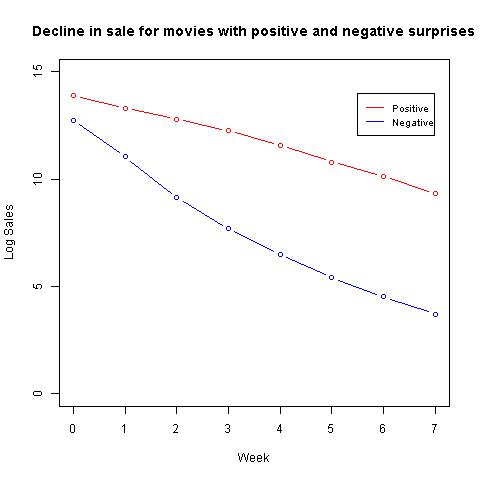
\includegraphics[scale=0.5]{plot_moretti.png}
\end{figure}
\begin{figure}\centering
	\label{part2.1_plot_fr}
	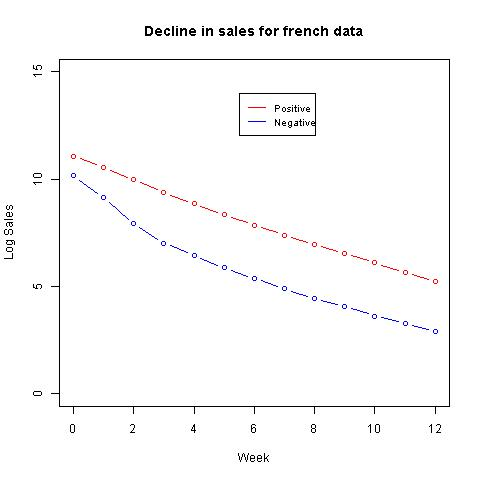
\includegraphics[scale=0.5]{plot_fr.png}
\end{figure}
\begin{figure}\centering
	\label{part2.1_plot_paris}
	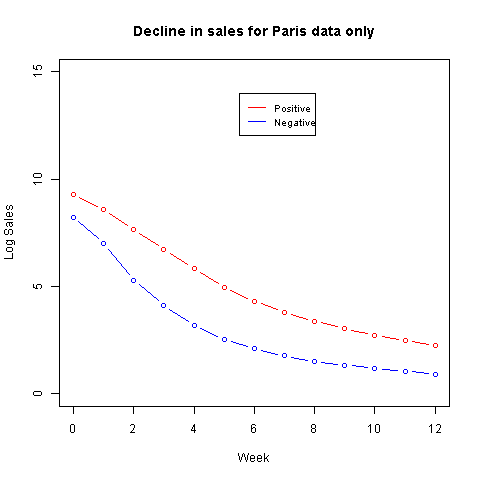
\includegraphics[scale=0.5]{plot_paris_only.png}
\end{figure}

% Table created by stargazer v.5.2 by Marek Hlavac, Harvard University. E-mail: hlavac at fas.harvard.edu
% Date and time: Wed, Feb 28, 2018 - 14:38:13
\begin{table}[!htbp] \centering 
	\caption{Decline in box-office sales by opening week surprise} 
	\label{} 
	\begin{tabular}{@{\extracolsep{5pt}}lcccc} 
		\\[-1.8ex]\hline 
		\hline \\[-1.8ex] 
		& \multicolumn{4}{c}{\textit{Dependent variable:}} \\ 
		\cline{2-5} 
		\\[-1.8ex] & \multicolumn{4}{c}{log\_sales} \\ 
		\\[-1.8ex] & (1) & (2) & (3) & (4)\\ 
		\hline \\[-1.8ex] 
		t & $-$0.952$^{***}$ & $-$0.952$^{***}$ & $-$1.289$^{***}$ &  \\ 
		& (0.007) & (0.006) & (0.009) &  \\ 
		& & & & \\ 
		t:surprise &  & 0.475$^{***}$ &  &  \\ 
		&  & (0.009) &  &  \\ 
		& & & & \\ 
		t:positive\_surprise &  &  & 0.640$^{***}$ &  \\ 
		&  &  & (0.013) &  \\ 
		& & & & \\ 
		I(t \textasteriskcentered  bottom\_surprise) &  &  &  & $-$1.353$^{***}$ \\ 
		&  &  &  & (0.011) \\ 
		& & & & \\ 
		I(t \textasteriskcentered  middle\_surprise) &  &  &  & $-$1.011$^{***}$ \\ 
		&  &  &  & (0.011) \\ 
		& & & & \\ 
		I(t \textasteriskcentered  top\_surprise) &  &  &  & $-$0.491$^{***}$ \\ 
		&  &  &  & (0.011) \\ 
		& & & & \\ 
		\hline \\[-1.8ex] 
		Observations & 39,936 & 39,936 & 39,936 & 39,936 \\ 
		R$^{2}$ & 0.772 & 0.788 & 0.787 & 0.790 \\ 
		Adjusted R$^{2}$ & 0.739 & 0.758 & 0.756 & 0.760 \\ 
		\hline 
		\hline \\[-1.8ex] 
		\textit{Note:}  & \multicolumn{4}{r}{$^{*}$p$<$0.1; $^{**}$p$<$0.05; $^{***}$p$<$0.01} \\ 
	\end{tabular} 
\end{table} 

% Table created by stargazer v.5.2 by Marek Hlavac, Harvard University. E-mail: hlavac at fas.harvard.edu
% Date and time: Wed, Feb 28, 2018 - 14:38:13
\begin{table}[!htbp] \centering 
	\caption{Precision of the prior} 
	\label{} 
	\begin{tabular}{@{\extracolsep{5pt}}lcc} 
		\\[-1.8ex]\hline 
		\hline \\[-1.8ex] 
		& \multicolumn{2}{c}{\textit{Dependent variable:}} \\ 
		\cline{2-3} 
		\\[-1.8ex] & \multicolumn{2}{c}{log\_sales} \\ 
		\\[-1.8ex] & (1) & (2)\\ 
		\hline \\[-1.8ex] 
		t & $-$1.291$^{***}$ & $-$1.267$^{***}$ \\ 
		& (0.010) & (0.087) \\ 
		& & \\ 
		t:positive\_surprise & 0.654$^{***}$ & $-$0.061 \\ 
		& (0.013) & (0.121) \\ 
		& & \\ 
		t:sequel & 0.037 &  \\ 
		& (0.038) &  \\ 
		& & \\ 
		t:positive\_surpriseTRUE:sequel & $-$0.225$^{***}$ &  \\ 
		& (0.053) &  \\ 
		& & \\ 
		t:var\_surprise &  & $-$0.045 \\ 
		&  & (0.174) \\ 
		& & \\ 
		t:positive\_surpriseTRUE:var\_surprise &  & 1.416$^{***}$ \\ 
		&  & (0.243) \\ 
		& & \\ 
		\hline \\[-1.8ex] 
		Observations & 39,936 & 39,936 \\ 
		R$^{2}$ & 0.787 & 0.787 \\ 
		Adjusted R$^{2}$ & 0.756 & 0.757 \\ 
		\hline 
		\hline \\[-1.8ex] 
		\textit{Note:}  & \multicolumn{2}{r}{$^{*}$p$<$0.1; $^{**}$p$<$0.05; $^{***}$p$<$0.01} \\ 
	\end{tabular} 
\end{table} 

FRANCE

% Table created by stargazer v.5.2 by Marek Hlavac, Harvard University. E-mail: hlavac at fas.harvard.edu
% Date and time: Wed, Feb 28, 2018 - 14:27:55
\begin{table}[!htbp] \centering 
	\caption{Decline in box-office sales by opening week surprise} 
	\label{} 
	\begin{tabular}{@{\extracolsep{5pt}}lcccc} 
		\\[-1.8ex]\hline 
		\hline \\[-1.8ex] 
		& \multicolumn{4}{c}{\textit{Dependent variable:}} \\ 
		\cline{2-5} 
		\\[-1.8ex] & \multicolumn{4}{c}{log\_entree\_fr} \\ 
		\\[-1.8ex] & (1) & (2) & (3) & (4)\\ 
		\hline \\[-1.8ex] 
		t & $-$0.526$^{***}$ & $-$0.526$^{***}$ & $-$0.571$^{***}$ &  \\ 
		& (0.002) & (0.002) & (0.003) &  \\ 
		& & & & \\ 
		t:surprise &  & 0.076$^{***}$ &  &  \\ 
		&  & (0.004) &  &  \\ 
		& & & & \\ 
		t:positive\_surprise &  &  & 0.087$^{***}$ &  \\ 
		&  &  & (0.004) &  \\ 
		& & & & \\ 
		t:bottom\_surpriseFALSE &  &  &  & $-$0.459$^{***}$ \\ 
		&  &  &  & (0.004) \\ 
		& & & & \\ 
		t:bottom\_surprise &  &  &  & $-$0.574$^{***}$ \\ 
		&  &  &  & (0.004) \\ 
		& & & & \\ 
		t:middle\_surprise &  &  &  & $-$0.088$^{***}$ \\ 
		&  &  &  & (0.005) \\ 
		& & & & \\ 
		\hline \\[-1.8ex] 
		Observations & 26,598 & 26,598 & 26,598 & 26,598 \\ 
		R$^{2}$ & 0.851 & 0.853 & 0.853 & 0.854 \\ 
		Adjusted R$^{2}$ & 0.838 & 0.841 & 0.841 & 0.841 \\ 
		\hline 
		\hline \\[-1.8ex] 
		\textit{Note:}  & \multicolumn{4}{r}{$^{*}$p$<$0.1; $^{**}$p$<$0.05; $^{***}$p$<$0.01} \\ 
	\end{tabular} 
\end{table} 

% Table created by stargazer v.5.2 by Marek Hlavac, Harvard University. E-mail: hlavac at fas.harvard.edu
% Date and time: Wed, Feb 28, 2018 - 14:27:56
\begin{table}[!htbp] \centering 
	\caption{Precision of the prior} 
	\label{} 
	\begin{tabular}{@{\extracolsep{5pt}}lccc} 
		\\[-1.8ex]\hline 
		\hline \\[-1.8ex] 
		& \multicolumn{3}{c}{\textit{Dependent variable:}} \\ 
		\cline{2-4} 
		\\[-1.8ex] & \multicolumn{3}{c}{log\_entree\_fr} \\ 
		\\[-1.8ex] & (1) & (2) & (3)\\ 
		\hline \\[-1.8ex] 
		t & $-$0.570$^{***}$ & $-$0.698$^{***}$ & $-$0.678$^{***}$ \\ 
		& (0.003) & (0.013) & (0.004) \\ 
		& & & \\ 
		t:positive\_surprise & 0.105$^{***}$ & 0.109$^{***}$ & 0.009 \\ 
		& (0.005) & (0.018) & (0.006) \\ 
		& & & \\ 
		t:saga & $-$0.027 &  &  \\ 
		& (0.016) &  &  \\ 
		& & & \\ 
		t:positive\_surpriseTRUE:saga & $-$0.145$^{***}$ &  &  \\ 
		& (0.019) &  &  \\ 
		& & & \\ 
		t:var\_surprise &  & 0.370$^{***}$ &  \\ 
		&  & (0.035) &  \\ 
		& & & \\ 
		t:positive\_surpriseTRUE:var\_surprise &  & $-$0.062 &  \\ 
		&  & (0.050) &  \\ 
		& & & \\ 
		t:art\_essai &  &  & 0.259$^{***}$ \\ 
		&  &  & (0.006) \\ 
		& & & \\ 
		t:positive\_surpriseTRUE:art\_essai &  &  & 0.066$^{***}$ \\ 
		&  &  & (0.008) \\ 
		& & & \\ 
		\hline \\[-1.8ex] 
		Observations & 26,598 & 26,546 & 26,598 \\ 
		R$^{2}$ & 0.855 & 0.854 & 0.880 \\ 
		Adjusted R$^{2}$ & 0.843 & 0.842 & 0.870 \\ 
		\hline 
		\hline \\[-1.8ex] 
		\textit{Note:}  & \multicolumn{3}{r}{$^{*}$p$<$0.1; $^{**}$p$<$0.05; $^{***}$p$<$0.01} \\ 
	\end{tabular} 
\end{table} 

PARIS

% Table created by stargazer v.5.2 by Marek Hlavac, Harvard University. E-mail: hlavac at fas.harvard.edu
% Date and time: Wed, Feb 28, 2018 - 14:37:16
\begin{table}[!htbp] \centering 
	\caption{Decline in box-office sales by opening week surprise} 
	\label{} 
	\begin{tabular}{@{\extracolsep{5pt}}lcccc} 
		\\[-1.8ex]\hline 
		\hline \\[-1.8ex] 
		& \multicolumn{4}{c}{\textit{Dependent variable:}} \\ 
		\cline{2-5} 
		\\[-1.8ex] & \multicolumn{4}{c}{log\_entree\_paris} \\ 
		\\[-1.8ex] & (1) & (2) & (3) & (4)\\ 
		\hline \\[-1.8ex] 
		t & $-$0.583$^{***}$ & $-$0.583$^{***}$ & $-$0.564$^{***}$ &  \\ 
		& (0.002) & (0.002) & (0.003) &  \\ 
		& & & & \\ 
		t:surprise &  & $-$0.032$^{***}$ &  &  \\ 
		&  & (0.004) &  &  \\ 
		& & & & \\ 
		t:positive\_surprise &  &  & $-$0.039$^{***}$ &  \\ 
		&  &  & (0.005) &  \\ 
		& & & & \\ 
		t:bottom\_surpriseFALSE &  &  &  & $-$0.594$^{***}$ \\ 
		&  &  &  & (0.004) \\ 
		& & & & \\ 
		t:bottom\_surprise &  &  &  & $-$0.541$^{***}$ \\ 
		&  &  &  & (0.004) \\ 
		& & & & \\ 
		t:middle\_surprise &  &  &  & $-$0.021$^{***}$ \\ 
		&  &  &  & (0.006) \\ 
		& & & & \\ 
		\hline \\[-1.8ex] 
		Observations & 35,113 & 35,113 & 35,113 & 35,113 \\ 
		R$^{2}$ & 0.810 & 0.810 & 0.810 & 0.811 \\ 
		Adjusted R$^{2}$ & 0.794 & 0.794 & 0.794 & 0.795 \\ 
		\hline 
		\hline \\[-1.8ex] 
		\textit{Note:}  & \multicolumn{4}{r}{$^{*}$p$<$0.1; $^{**}$p$<$0.05; $^{***}$p$<$0.01} \\ 
	\end{tabular} 
\end{table} 

% Table created by stargazer v.5.2 by Marek Hlavac, Harvard University. E-mail: hlavac at fas.harvard.edu
% Date and time: Wed, Feb 28, 2018 - 14:37:16
\begin{table}[!htbp] \centering 
	\caption{Precision of the prior} 
	\label{} 
	\begin{tabular}{@{\extracolsep{5pt}}lccc} 
		\\[-1.8ex]\hline 
		\hline \\[-1.8ex] 
		& \multicolumn{3}{c}{\textit{Dependent variable:}} \\ 
		\cline{2-4} 
		\\[-1.8ex] & \multicolumn{3}{c}{log\_entree\_paris} \\ 
		\\[-1.8ex] & (1) & (2) & (3)\\ 
		\hline \\[-1.8ex] 
		t & $-$0.560$^{***}$ & $-$0.772$^{***}$ & $-$0.616$^{***}$ \\ 
		& (0.003) & (0.017) & (0.005) \\ 
		& & & \\ 
		t:positive\_surprise & $-$0.030$^{***}$ & $-$0.213$^{***}$ & $-$0.126$^{***}$ \\ 
		& (0.005) & (0.024) & (0.007) \\ 
		& & & \\ 
		t:saga & $-$0.118$^{***}$ &  &  \\ 
		& (0.017) &  &  \\ 
		& & & \\ 
		t:positive\_surpriseTRUE:saga & $-$0.022 &  &  \\ 
		& (0.020) &  &  \\ 
		& & & \\ 
		t:var\_surprise &  & 0.576$^{***}$ &  \\ 
		&  & (0.045) &  \\ 
		& & & \\ 
		t:positive\_surpriseTRUE:var\_surprise &  & 0.480$^{***}$ &  \\ 
		&  & (0.065) &  \\ 
		& & & \\ 
		t:art\_essai &  &  & 0.087$^{***}$ \\ 
		&  &  & (0.006) \\ 
		& & & \\ 
		t:positive\_surpriseTRUE:art\_essai &  &  & 0.156$^{***}$ \\ 
		&  &  & (0.009) \\ 
		& & & \\ 
		\hline \\[-1.8ex] 
		Observations & 35,113 & 35,074 & 35,113 \\ 
		R$^{2}$ & 0.811 & 0.814 & 0.819 \\ 
		Adjusted R$^{2}$ & 0.795 & 0.798 & 0.804 \\ 
		\hline 
		\hline \\[-1.8ex] 
		\textit{Note:}  & \multicolumn{3}{r}{$^{*}$p$<$0.1; $^{**}$p$<$0.05; $^{***}$p$<$0.01} \\ 
	\end{tabular} 
\end{table} 

\subsection{Precision of the prior}

\subsection{Size of the Social Network}\label{subsec2.4}

Consumers with a larger social network receive more feedbacks from their peers and thus they are able to evaluate more precisely the quality of the movie.
Hence, social learning should be stronger for consumers with a larger social network.
More formally, this prediction can be tested by estimating the models of the form:
\begin{equation}
	\ln (y_{jt})  = \beta_0 + \beta_1 t + \beta_2 (t \times S_j) + \beta_3 (t \times NS_j) + \beta_4 (t \times S_j \times NS_j) + d_j + u_{jt}
	\label{eqpred3}
\end{equation}
where $S_j$ is a dummy for positive surprise and $NS_j$ is a variable representing the network size of the movie $j$'s audience.
If social learning is stronger with higher values of $NS_j$, then the coefficient $\beta_4$ of the triple interaction between the time trend, the surprise and the network size should be positive.

In his article, Moretti uses two different measurement of network size.
First, he makes the assumption that teenagers have a more developed social network than adults and he estimates the model of equation \ref{eqpred3} with a dummy for teen movies.
He finds that the estimate of the coefficient $\beta_4$ is indeed positive.
However, the estimate is very weakly significant.
Additionally, there is no indicator for teen movies in the data and the way Moretti build a dummy for teen movies is quite surprising.
He uses \textit{genre1} (one of the three variables indicating the genre of the movies) and he considers that teen movies are movies of the genre action, adventure, comedy, fantasy, horror, sci-fi and suspense.
We would have appreciated more justification for the assumption that teenagers have a larger social network and for the way teen movies are defined.
To investigate further these issues, we used the two other variables indicating the genre of the movies: \textit{genre2} and \textit{genre3}.
Both variables have a category \textit{Children} and a category \textit{Youth}.
We used these two categories to define new dummies for teen movies.
Using \textit{genre2}, we find that the estimate of $\beta_4$ is significantly negative.
Using \textit{genre3}, we find that the estimate of $\beta_4$ is significantly positive.
We conclude that using teen movies is not a good way to test this prediction.

A second measurement of the size of the social network used by Moretti is the number of theaters broadcasting the movie during the opening week.
If a movie opens in lots of theater, the consumers should receive more feedbacks from their peers.
As expected, he estimates that the coefficient of $\beta_4$ is significantly positive.
We estimated the same model with the French data.
The results are reported in column (2) of table \ref{precisionsignal}.
We find that the coefficient of the triple interaction is indeed significantly positive.

In the French data, the variable \textit{tout public} is a dummy indicating movies which are suitable for any kind of audience.
We can assume that consumers have more feedbacks from their peers for movies opened to anyone.
Hence, we estimated the model of equation \ref{eqpred3} using the \textit{tout public} dummy to measure network size.
The results of the estimated are reported in column (1) of table \ref{precisionsignal}.
Consistently with our assumption, the coefficient of the triple interaction is significantly positive.

% Table created by stargazer v.5.2 by Marek Hlavac, Harvard University. E-mail: hlavac at fas.harvard.edu
% Date and time: Fri, Mar 02, 2018 - 05:12:24 PM
\begin{table}[!htbp] \centering 
  \caption{Precision of peers' signal} 
  \label{precisionsignal} 
\begin{tabular}{@{\extracolsep{5pt}}lcc} 
\\[-1.8ex]\hline 
\hline \\[-1.8ex] 
 & \multicolumn{2}{c}{\textit{Dependent variable:}} \\ 
\cline{2-3} 
\\[-1.8ex] & \multicolumn{2}{c}{log\_entree\_fr} \\ 
\\[-1.8ex] & (1) & (2)\\ 
\hline \\[-1.8ex] 
 $t$ & $-$0.663$^{***}$ & $-$0.451$^{***}$ \\ 
  & (0.007) & (0.005) \\ 
  & & \\ 
 $t$$\times$positive\_surprise & 0.061$^{***}$ & 0.076$^{***}$ \\ 
  & (0.010) & (0.006) \\ 
  & & \\ 
 $t$$\times$tout\_public & 0.115$^{***}$ &  \\ 
  & (0.008) &  \\ 
  & & \\ 
 $t$$\times$positive\_surprise$\times$tout\_public & 0.031$^{***}$ &  \\ 
  & (0.011) &  \\ 
  & & \\ 
 $t$$\times$seance\_fr\_first\_week &  & $-$0.033$^{***}$ \\ 
  &  & (0.001) \\ 
  & & \\ 
 $t$$\times$positive\_surprise$\times$seance\_fr\_first\_week &  & 0.011$^{***}$ \\ 
  &  & (0.001) \\ 
  & & \\ 
\hline \\[-1.8ex] 
Observations & 26,598 & 26,598 \\ 
R$^{2}$ & 0.856 & 0.867 \\ 
Adjusted R$^{2}$ & 0.844 & 0.856 \\ 
\hline 
\hline \\[-1.8ex] 
\textit{Note:}  & \multicolumn{2}{r}{$^{*}$p$<$0.1; $^{**}$p$<$0.05; $^{***}$p$<$0.01} \\ 
\end{tabular} 
\end{table}

\subsection{Does learning decline over time?}\label{subsec2.5}

The model predicts that the effects of positive and negative surprises should decline over time.
More precisely, sales profile should be a concave function of time for positive surprises and a convex function of time for negative surprises.
To test this prediction, we need to estimate the sales profile which is assumed to be a quadratic function of time.
Therefore, we estimate the following model:
\begin{equation*}
	\ln (y_{jt}) = \beta_0 + \beta_1 t + \beta_2 t^2 + \beta_3 (t \times S_j) + \beta_4 (t^2 \times S_j) + d_j + u_{jt}
\end{equation*}
where $S_j$ is a dummy for positive surprise.
The results are reported in table \ref{pred4}.
The second derivative of log of entries for negative-surprise movies is 
\begin{equation*}
	\left.\frac{\partial^2 y_{jt}}{\partial t^2}\right|_{S_j=0} = 2 \beta_2.
\end{equation*}
The second derivative of log of entries for positive-surprise movies is 
\begin{equation*}
	\left.\frac{\partial^2 y_{jt}}{\partial t^2}\right|_{S_j=1} = 2 (\beta_2 + \beta_4).
\end{equation*}
We can test the hypothesis of convexity ($2\beta_2 > 0$) and the hypothesis of concavity ($2(\beta_2 + \beta_4) < 0$) with Student tests.
For instance, to test $H_0:~2(\beta_2 + \beta_4) < 0$ against $H_1:~2(\beta_2 + \beta_4) > 0$, the $t$ statistic is
\begin{equation*}
	t = \frac{2(\hat{\beta}_2 + \hat{\beta}_4)}{\text{se}(2(\hat{\beta}_2 + \hat{\beta}_4))} 
\end{equation*}
where $\text{se}(2(\hat{\beta}_2 + \hat{\beta}_4)) = 2[\text{Var}(\hat{\beta}_2) + \text{Var}(\hat{\beta}_4) + 2\cdot \text{Cov}(\hat{\beta}_2, \hat{\beta}_4)]^{1/2}$ is the standard error of $2(\hat{\beta}_2 + \hat{\beta}_4)$.

With the US data, both hypotheses cannot be rejected with a good confidence.
With French data, the $p$-value for the test of convexity of negative-surprise movies is really close to 0 ($t \approx 36.72$ and $p \approx 0$). 
However, the hypothesis of concavity of positive-surprise movies must be rejected ($t \approx 9.41$ and $p \approx 1$).
What we can say however is that the sales profile of positive-surprise movies is \textit{more concave} than the sales profile of negative-surprise movies because the estimates show that the coefficient $\beta_4$ is significantly negative.
These statements are confirmed by the graphs of the sales profile of figure \ref{part2.1_plot_moretti} where the sales profile of negative-surprise movies is clearly convex and the sales profile of positive-surprise movies seems linear.

% Table created by stargazer v.5.2 by Marek Hlavac, Harvard University. E-mail: hlavac at fas.harvard.edu
% Date and time: Fri, Mar 02, 2018 - 05:12:25 PM
\begin{table}[!htbp] \centering 
  \caption{Convexity of the sales profile} 
  \label{pred4} 
\begin{tabular}{@{\extracolsep{5pt}}lc} 
\\[-1.8ex]\hline 
\hline \\[-1.8ex] 
 & \multicolumn{1}{c}{\textit{Dependent variable:}} \\ 
\cline{2-2} 
\\[-1.8ex] & log\_entree\_fr \\ 
\hline \\[-1.8ex] 
 $t$ & $-$0.978$^{***}$ \\ 
  & (0.011) \\ 
  & \\ 
 $t^2$ & 0.034$^{***}$ \\ 
  & (0.001) \\ 
  & \\ 
 $t$$\times$positive\_surprise & 0.393$^{***}$ \\ 
  & (0.016) \\ 
  & \\ 
 $t^2$$\times$positive\_surprise & $-$0.026$^{***}$ \\ 
  & (0.001) \\ 
  & \\ 
\hline \\[-1.8ex] 
Observations & 26,598 \\ 
R$^{2}$ & 0.861 \\ 
Adjusted R$^{2}$ & 0.850 \\ 
\hline 
\hline \\[-1.8ex] 
\textit{Note:}  & \multicolumn{1}{r}{$^{*}$p$<$0.1; $^{**}$p$<$0.05; $^{***}$p$<$0.01} \\ 
\end{tabular} 
\end{table}

\section{Conclusion}
%\pagebreak
%\begin{appendices}
%\section{R codes}
%\paragraph{Data cleaning}
%\begin{figure}[H]
	%\caption{R code used to clean French data}
	%\label{code_data_cleaning}
	%\begin{lstlisting}
	%###################
	%#  Data Cleaning  #
	%###################
	%
	%# In this part, we change the dataset to make it closer to the dataset of Moretti.
	%
	%# Remove the movies without any screen in France during the first week (667 movies).
	%fr_df <- fr_df[!is.na(fr_df$seance_fr1),]
	%# Remove the movies without any id_distributeur (4 movies).
	%fr_df <- fr_df[!is.na(fr_df$id_distributeur),]
	%
	%# Set MoyennePresse and MoyenneSpectateur to the mean if no value is specified.
	%mean_moy <- mean(fr_df[!is.na(fr_df$MoyennePresse), 'MoyennePresse'])
	%fr_df[is.na(fr_df$MoyennePresse), 'MoyennePresse'] <- mean_moy
	%mean_moy <- mean(fr_df[!is.na(fr_df$MoyenneSpectateur), 'MoyenneSpectateur'])
	%fr_df[is.na(fr_df$MoyenneSpectateur), 'MoyenneSpectateur'] <- mean_moy
	%
	%# Repeat each columns 13 times.
	%n <- nrow(fr_df)
	%df <- fr_df[rep(1:n, each=13),]
	%
	%# Add a column to indicate the week.
	%df$t <- rep(0:12, n)
	%
	%# Replace the variables for each week (e.g. 'entree_paris1') with a global variable (e.g. 'entree_paris')
	%for (i in 0:12) {
	%for (variable in c('entree_paris', 'seance_paris', 'entree_fr', 'seance_fr')) {
	%# Concatenate the variable name with and indicator for the week (e.g. 'entree_paris1').
	%variable_t <- paste(c(variable, toString(i+1)), collapse='')
	%# For each week, the variable in the new df (e.g. 'entree_paris') is taken from the old df (e.g. 'entree_paris1').
	%df[df$t==i, variable] <- fr_df[,variable_t]
	%}
	%}
	%
	%# Keep only the useful variables.
	%df <- df[,c(1:6, 33:43, 70:85)]
	%
	%# Replace the NAs in seance_fr with zeros.
	%df[is.na(df$seance_fr), 'seance_fr'] <- 0
	%
	%# Generate logarithm of sales and screens.
	%df$log_entree_paris <- log(df$entree_paris + 1)
	%df$log_seance_paris <- log(df$seance_paris + 1)
	%df$log_entree_fr <- log(df$entree_fr + 1)
	%df$log_seance_fr <- log(df$seance_fr + 1)
	%
	%# Variable id_distributeur is a factor.
	%df$id_distributeur <- as.factor(df$id_distributeur)
	%
	%# Variable id is a factor (this is used for movie dummies with the package lfe).
	%df$X <- as.factor(df$X)
	%df$X.eff <- rnorm(nlevels(df$X))
	%
	%\end{lstlisting}
%\end{figure}
%\begin{figure}[H]
	%\caption{R code used to obtain French surprises}
	%\label{code_french_surprises}
	%\begin{lstlisting}
	%###############
	%#  Surprises  #
	%###############
	%
	%# In this part, we estimate the surprises of the movies.
	%
	%# Regression of first week sales on number of screens.
	%regSurprise1 <- lm(log_entree_fr ~ log_seance_fr, data = df, subset = (t==0))
	%# Including dummies for genre
	%regSurprise2 <- lm(log_entree_fr ~ log_seance_fr + genre, data = df, subset = (t==0))
	%# Including dummies for ratings 
	%regSurprise3 <- lm(log_entree_fr ~ log_seance_fr + genre + interdiction, data = df, subset = (t==0))
	%# Including dummies for distributor 
	%regSurprise4 <- lm(log_entree_fr ~ log_seance_fr + genre + interdiction + id_distributeur, data = df, subset = (t==0))
	%# Including dummies for month and week 
	%regSurprise5 <- lm(log_entree_fr ~ log_seance_fr + genre + interdiction + id_distributeur + factor(mois) + factor(semaine), data = df, subset = (t==0))
	%# Including dummies for year 
	%regSurprise6 <- lm(log_entree_fr ~ log_seance_fr + genre + interdiction + id_distributeur + factor(mois) + factor(semaine) + factor(annee), data = df, subset = (t==0))
	%# Including other variables
	%regSurprise7 <- lm(log_entree_fr ~ log_seance_fr + genre + interdiction + id_distributeur + factor(mois) + factor(semaine) + factor(annee) + MoyennePresse + sigma_note_presse + PoidsCasting + pub, data = df, subset = (t==0))
	%
	%# Print a table with the results of the last regressions.
	%stargazer(regSurprise1, regSurprise2, regSurprise3, regSurprise4, regSurprise5, regSurprise6, regSurprise7, type='text', keep=c('log_seance_fr'), omit.stat=c("f", "ser"), title='Regression of first-week entries on number of screens')
	%
	%# Surprises are defined as the residuals of the last regression.
	%surprise <- residuals(regSurprise7)
	%df$surprise <- rep(residuals(regSurprise3), each = 13)
	%quantile(df$surprise, probs = c(0, .05, .1, .25, .5, .75, .9, .95, 1))
	%
	%# Generate additional variables for surprises.
	%df$positive_surprise <- df$surprise >= 0
	%q_surprise <- quantile(df$surprise, probs = c(1/3, 2/3))
	%df$bottom_surprise <- df$surprise < q_surprise[1]
	%df$middle_surprise <- df$surprise >= q_surprise[1] & df$surprise < q_surprise[2]
	%df$top_surprise <- df$surprise >= q_surprise[2]
	%
	%\end{lstlisting}
%\end{figure}
%
%\begin{figure}[H]
	%\caption{R code used to obtain French sales dynamics}
	%\label{code_}
	%\begin{lstlisting}
	%###############################################
	%#  Prediction 1: Surprises and Sale Dynamics  #
	%###############################################
	%
	%# In this part, we study the difference in rate of decline between movies with a positive surprise and movies with a negative surprise.
	%
	%# Regression of sales on the interaction between time and surprises.
	%# We use the command felm of the package lfe to compute linear regressions with thousands of dummies.
	%regSaleDynamics1 <- felm(log_entree_fr ~ t | X, data = df)
	%regSaleDynamics2 <- felm(log_entree_fr ~ t + t : surprise | X, data = df)
	%regSaleDynamics3 <- felm(log_entree_fr ~ t + t : positive_surprise | X, data = df)
	%regSaleDynamics4 <- felm(log_entree_fr ~ I(t * top_surprise)+ I(t * middle_surprise) + I(t * bottom_surprise) | X, data = df)
	%
	%# Print a table with the results of the regressions.
	%stargazer(regSaleDynamics1, regSaleDynamics2, regSaleDynamics3, regSaleDynamics4, omit.stat=c("f", "ser"), title='Decline in box-office sales by opening week surprise')
	%
	%
	%\end{lstlisting}
	%
	%
%\end{figure}
%
%
%
%
%
%
%
%
%
%
%
%
%\end{appendices}



\end{document}
